\documentclass[
  oneside,
  11pt, a4paper,
  footinclude=true,
  headinclude=true,
  cleardoublepage=empty
]{article}

\usepackage{lipsum}
\usepackage{amsmath}
\usepackage{amsthm}
\usepackage{acronym}
\usepackage{hyperref}
\usepackage{graphicx}
\usepackage{apacite}
\usepackage{natbib}
\usepackage{caption}
\usepackage{subcaption}
\usepackage[utf8]{inputenc}
\graphicspath{{images/}}

\title{Virtour: Telepresence System for Remotely Operated Building Tours}
\author{Patricio Lankenau\\
        University of Texas at Austin, Austin, Texas\\
        patricio.lankenau@utexas.edu\\}
\date{August 11, 2016}

\begin{document}

\maketitle

\begin{abstract}
  In this paper we describe Virtour, a public facing system for teleoperated
  building tours. It aims to facilitate lab and departmental tours by creating
  a system wherein prospective students can remotely operate a wheeled robot
  around the Building-Wide Intelligence lab and the rest of the computer
  science building. Virtour's server architecture builds on the existing
  Building-Wide Intelligence autonomous robot platform, which is capable of
  autonomous localization, planning, and navigation. The web client interface
  is built using modern web technologies to allow users to control our robots
  from any internet device (e.g., cellphone, tablet, computer). Virtour
  provides an interface where users can view what the robot sees, as well as
  control the robot's rotation and camera angle in real time. Navigation is
  provided using a map where users can select their desired destination and
  have the robot autonomously navigate there. This approach eliminates the risk
  of human navigation error by abstracting away movement commands. As a result
  we can provide users an immersive telepresence system, which is safe to use,
  and provides a service to our lab and department by allowing anyone to visit
  to experience the areas first-hand.
\end{abstract}

\vfill

\subsubsection*{\centering In fulfillment of the Turing Scholars Honors Thesis
requirement}

\subsubsection*{\centering Advisor: Peter Stone}

%\tableofcontents
\newpage

\section{Introduction}\label{sec:intro}

The University of Texas at Austin has a constant stream of visitors and tours
of the campus. Of special interest to us are the large number of tours given at
our computer science building. The tour guests range in ages and backgrounds,
and tend to be prospective students to both undergraduate and graduate programs,
or visiting faculty. Unfortunately, there is a large population of prospective
students that are unable to physically come to our campus and are thus unable
to partake in the conventional tours.

We designed Virtour to address this problem. Virtour is a public facing system
for teleoperated building tours. Virtour builds on the existing Building-Wide
Intelligence (BWI) autonomous robot platform. It utilizes the lab's autonomous
wheeled robots which can localize, navigate, and perform tasks without human
intervention for long periods of time. Through the use of modern web and robot
technologies, Virtour allows untrained public users to remotely control our
robots in what we call a virtual tour. Our system is created under the
principle of shared autonomy, which aims to balance external control abilities
while maintaining our rigorous standard of safety and security for the robots
and people involved. As such, it provides the user control over what the robot
is doing, while simultaneously using the existing the autonomous navigation
capabilities and obstacle avoidance to ensure safety and correct operation.

The two major contributions of this work are as follows. First, we present the
server framework as described in Section \ref{sec:server}. This is system can
be extended and used to expose arbitrary robot capabilities to the internet,
and can be used for much more than just campus tours. Furthermore, this system
was built with security in mind, as described in Section \ref{sec:security},
which makes it secure for public web deployment. Our second contribution is the
novel approach to the user interface client, which is designed to be accessible
by all modern internet-capable devices and adheres to modern web 2.0 standards,
as described in Section \ref{sec:client}.

\section{Related Work}\label{sec:related}

Web-based tours have been an active area of research in the past. The earliest
virtual tour system was built to serve as a museum tour guide in 1998 by
\citet{burgard1998}. Their robot, Rhino, operated mainly as a physically
interactive tour guide that museum visitors could approach and request tours
from, but also supported occasional web-based tours where online visitors could
vote on defined tours to spectate. Their web-based interface provided images from
the on-board camera as well as static cameras placed throughout the museum, and
allowed the user to download a Java applet to see real-time information. Web
control was limited to voting on a desired tour (from a pre-programmed list)
and viewing the robot's image stream.

Later work introduced a second-generation museum tour-guide robot by
\citet{thrun1999} named Minerva, which improved on the work done by Burgard.
Most of their improvements were in the areas of localization, mapping,
simultaneous localization and mapping (SLAM), and human robot interaction
(HRI). They improved the virtual tour interface by allowing arbitrary selection
of navigation goals, rather than a pre-selected list. However, web control was
still limited and their real-time information display required the download of
a Java web-applet.

\citet{kim2004} developed Jinny in 2004, which was yet another autonomous
tour-guide robot. Their relevant contribution was the upgraded web-based
interface which allowed the user to interact with a natural language parsing
system to ask questions, as well as request actions. Their system is built
using Java and ActiveX, both of which require special installation for the
users.

Virtour differs from these related works in a number of ways. The first is that
Virtour's main purpose is to be a telepresence tour system, and thus gives web
visitors priority in controlling the robot (unlike Rhino or Minerva, which only
occasionally allow web control). Our web client is unique in that it uses only
modern web standards and does not require the end-user to download any extra
software (e.g., Java, ActiveX). Thus, Virtour is truly portable and can accessed
from any web-connected modern device. Virtour is also unique in that it
provides the end-user with real-time video feedback and information about the
robot. For example, the robot's position is updated on the website in
real-time without requiring any additional simulation software. Furthermore,
the user's actions are performed in real-time and the results are shown almost
immediately; therefore, if a user request for the robot to rotate, he or she will be
able to see the robot's camera feed update instantly. As part of Virtour's
goal of ease of use, it uses bandwidth scaling of video streaming to reduce the
quality of the video according to the end-user's internet connection. Finally,
Virtour is novel because it provides the end user with a wide variety of ways
of interacting with the robot. Rather than just providing navigation and video
streaming, it allows the user to deliver spoken messages and perform tasks.

\section{Building Wide Intelligence}\label{sec:bwi}

Virtour is a part of the Building Wide Intelligence (BWI) project, which aims
to develop fully-autonomous mobile robots that exists as permanent inhabitants
of UT's Computer Science departmental building. The BWI project lies in the
intersection of Artificial Intelligence and Robotics, and works to create
robots that are useful as research platforms, as well as helpful to the humans
in the building.

Virtour runs on the BWI segbot robot platform --- our in-house robot platform
which has been in development for over four years. Currently, our lab has four
active robots. Three of the robots are based on the older generation hardware
and software (Version 2 as depicted in Figure \ref{fig:segbotv2}) one of which
is also equipped with a Kinova Mico Arm\footnote{This version of the Kinova arm
has 6 degrees of freedom, a reach of 700 mm, and a mid-range payload capacity
of 2.1 kg} (shown in Figure \ref{fig:segbotarm}). We have one Version 3 robot
(depicted in Figure \ref{fig:segbotv3}), which has been our pilot test as we
transition all our robots to new hardware and software. Virtour supports both
platform versions, and will adapt its features accordingly (based on which
robot you connect to). However, since Virtour is mostly used on the Version 3
robot, we will only describe the latest hardware platform.

\begin{figure}[!tbp]
  \begin{subfigure}[b]{0.3\textwidth}
    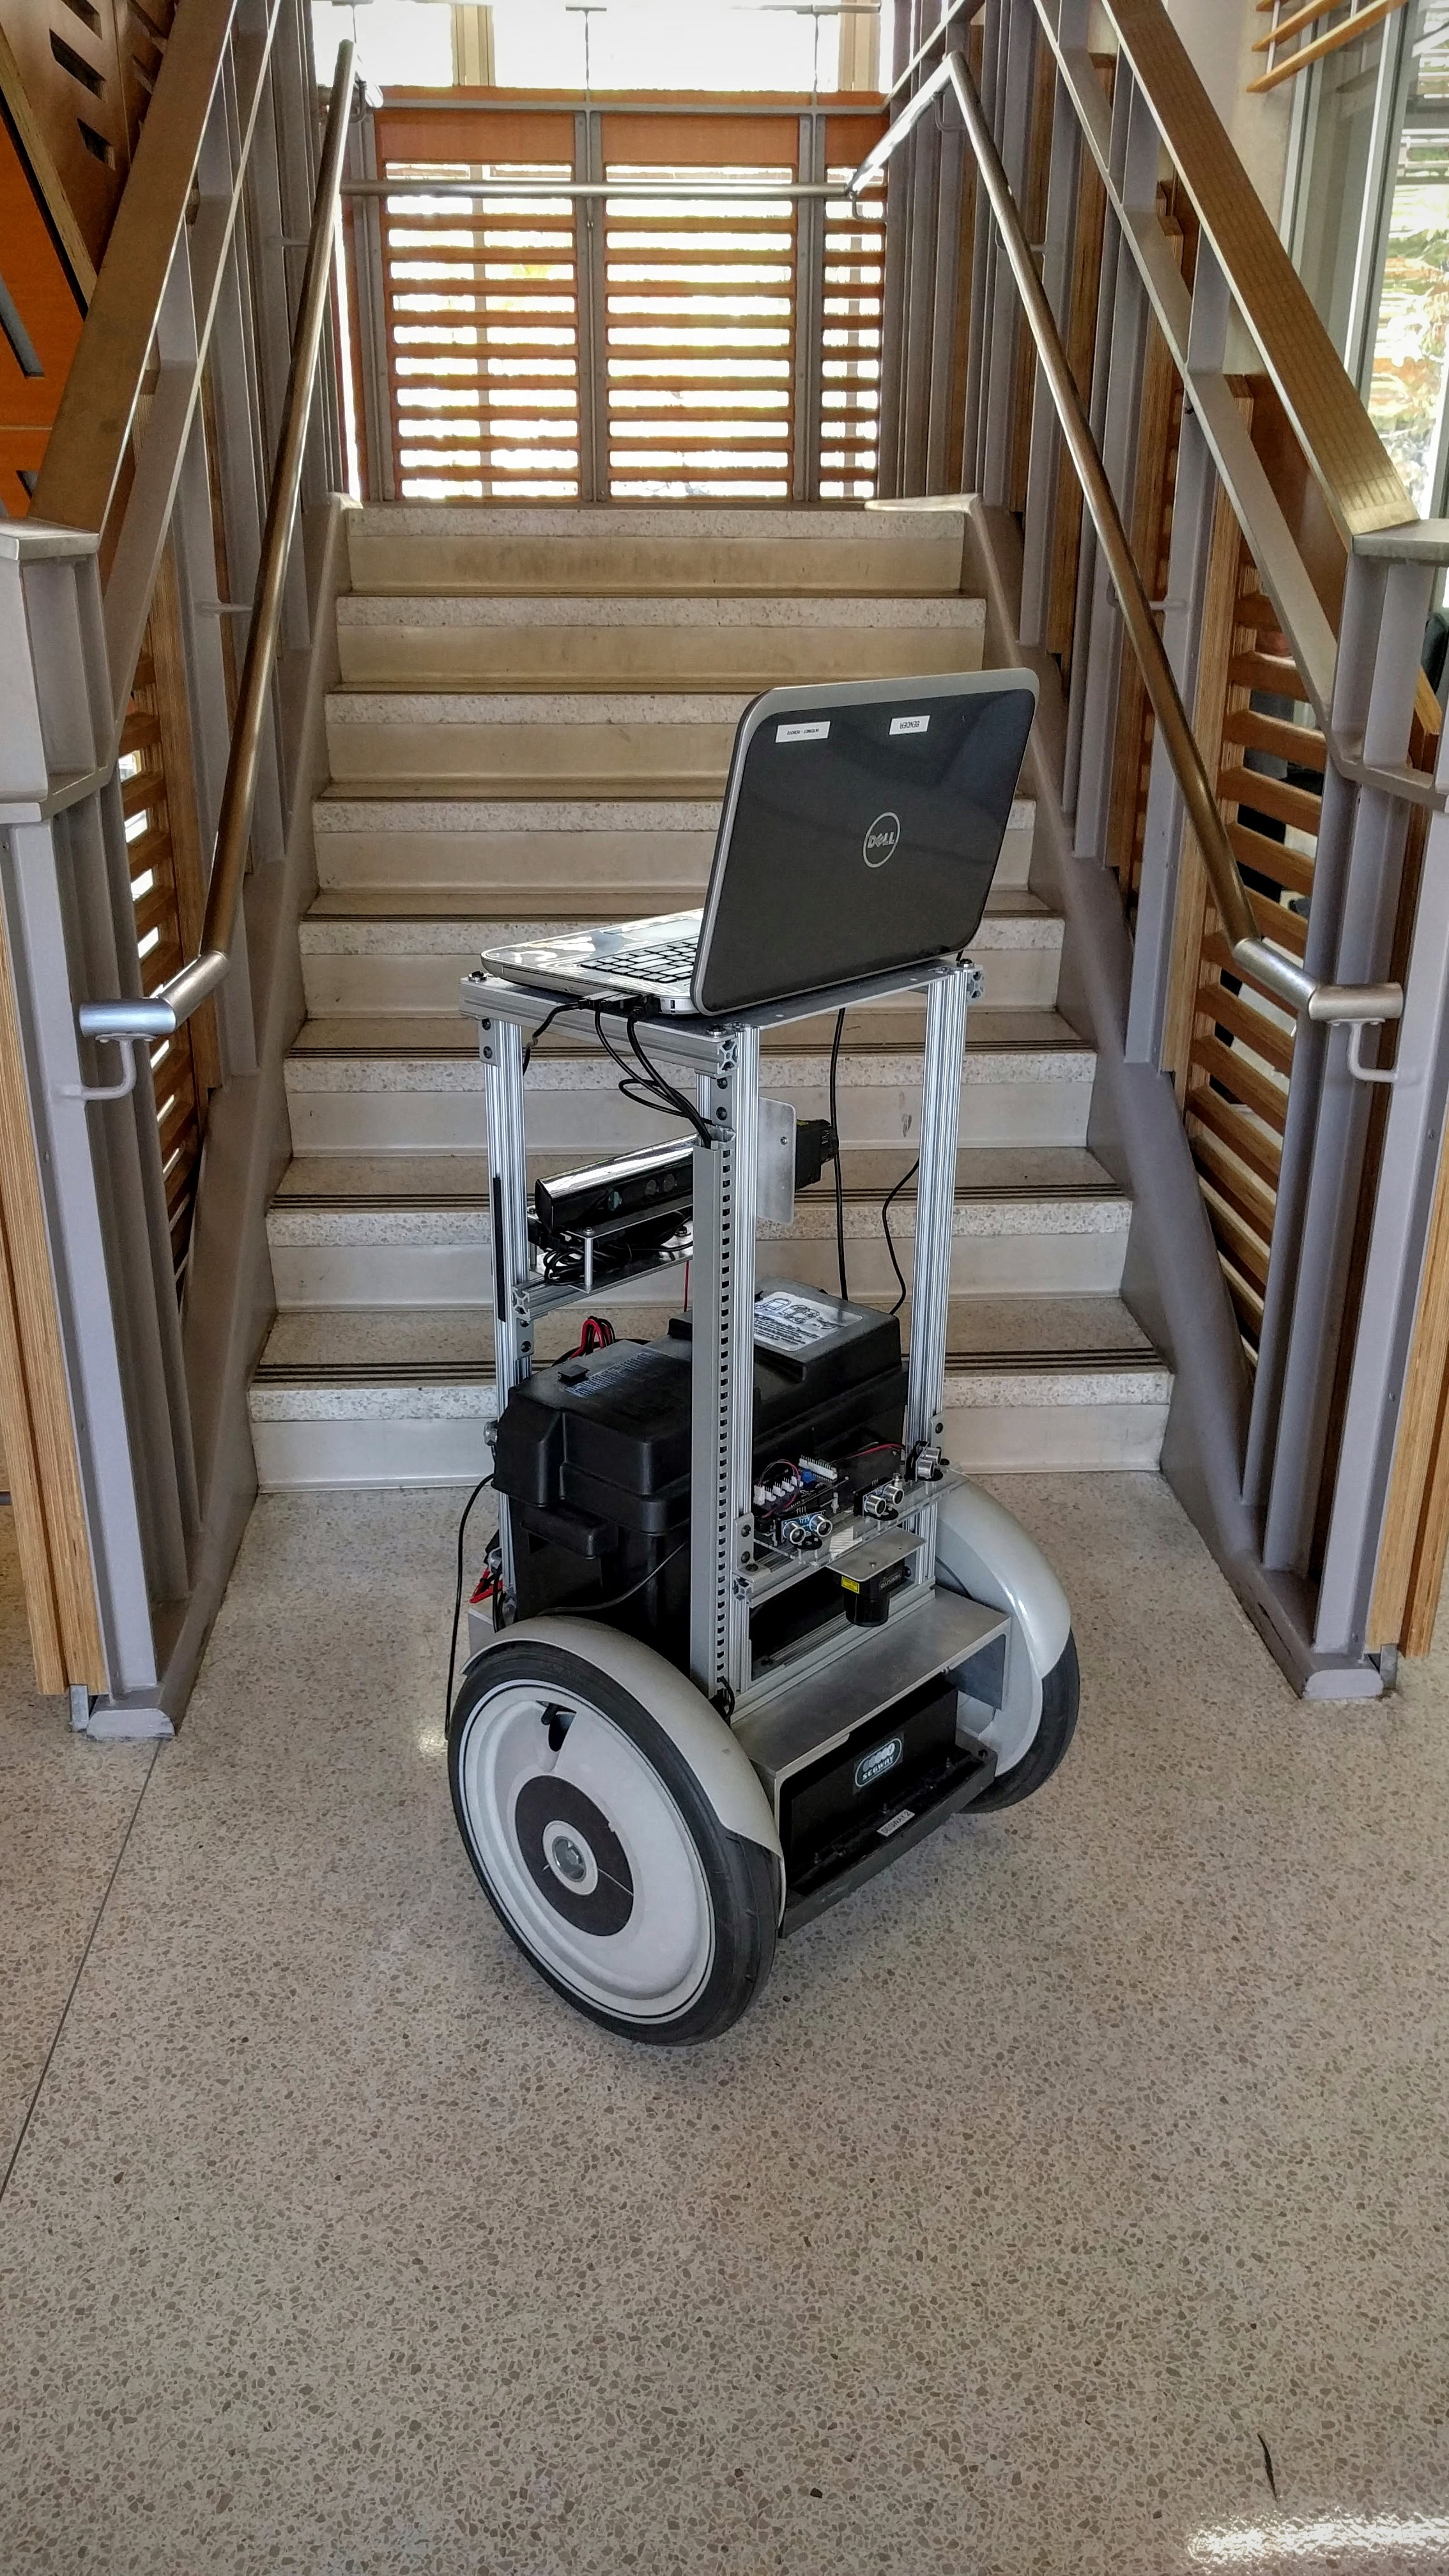
\includegraphics[width=\textwidth]{bwi_segbot2}
    \caption{Segbot v2}
    \label{fig:segbotv2}
  \end{subfigure}
  \hfill
  \begin{subfigure}[b]{0.3\textwidth}
    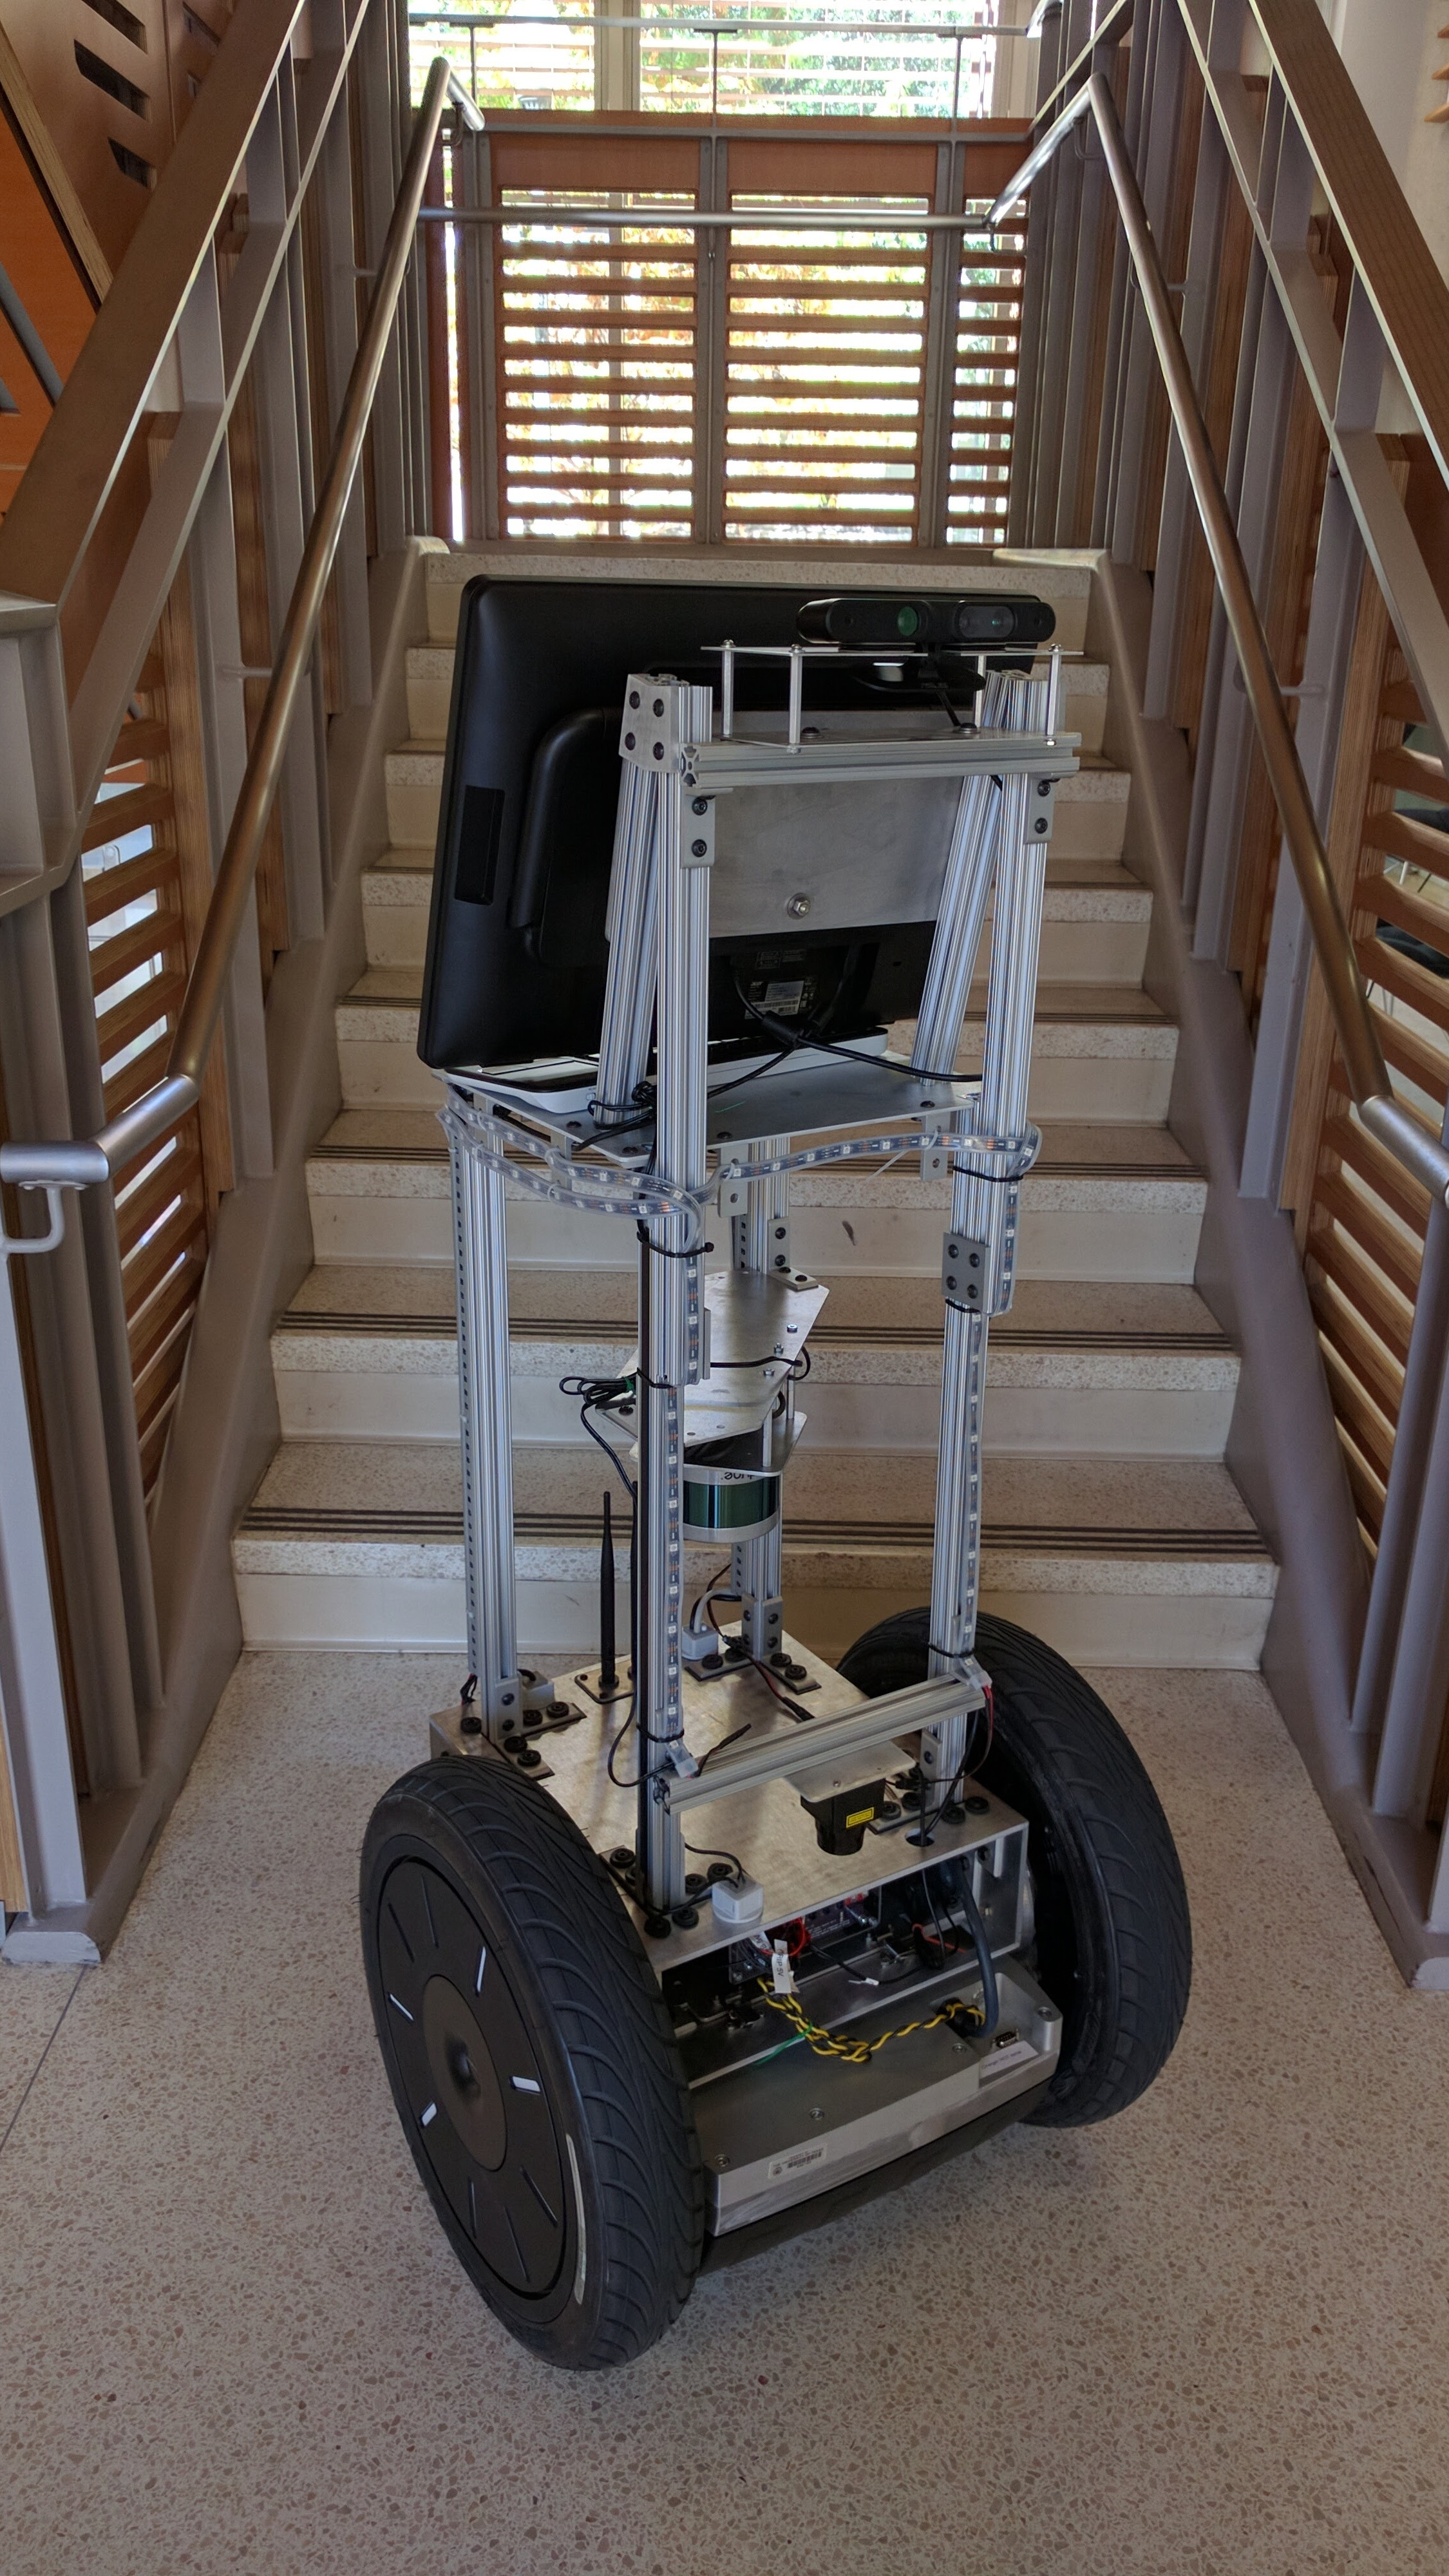
\includegraphics[width=\textwidth]{bwi_segbot3}
    \caption{Segbot v3}
    \label{fig:segbotv3}
  \end{subfigure}
  \hfill
  \begin{subfigure}[b]{0.3\textwidth}
    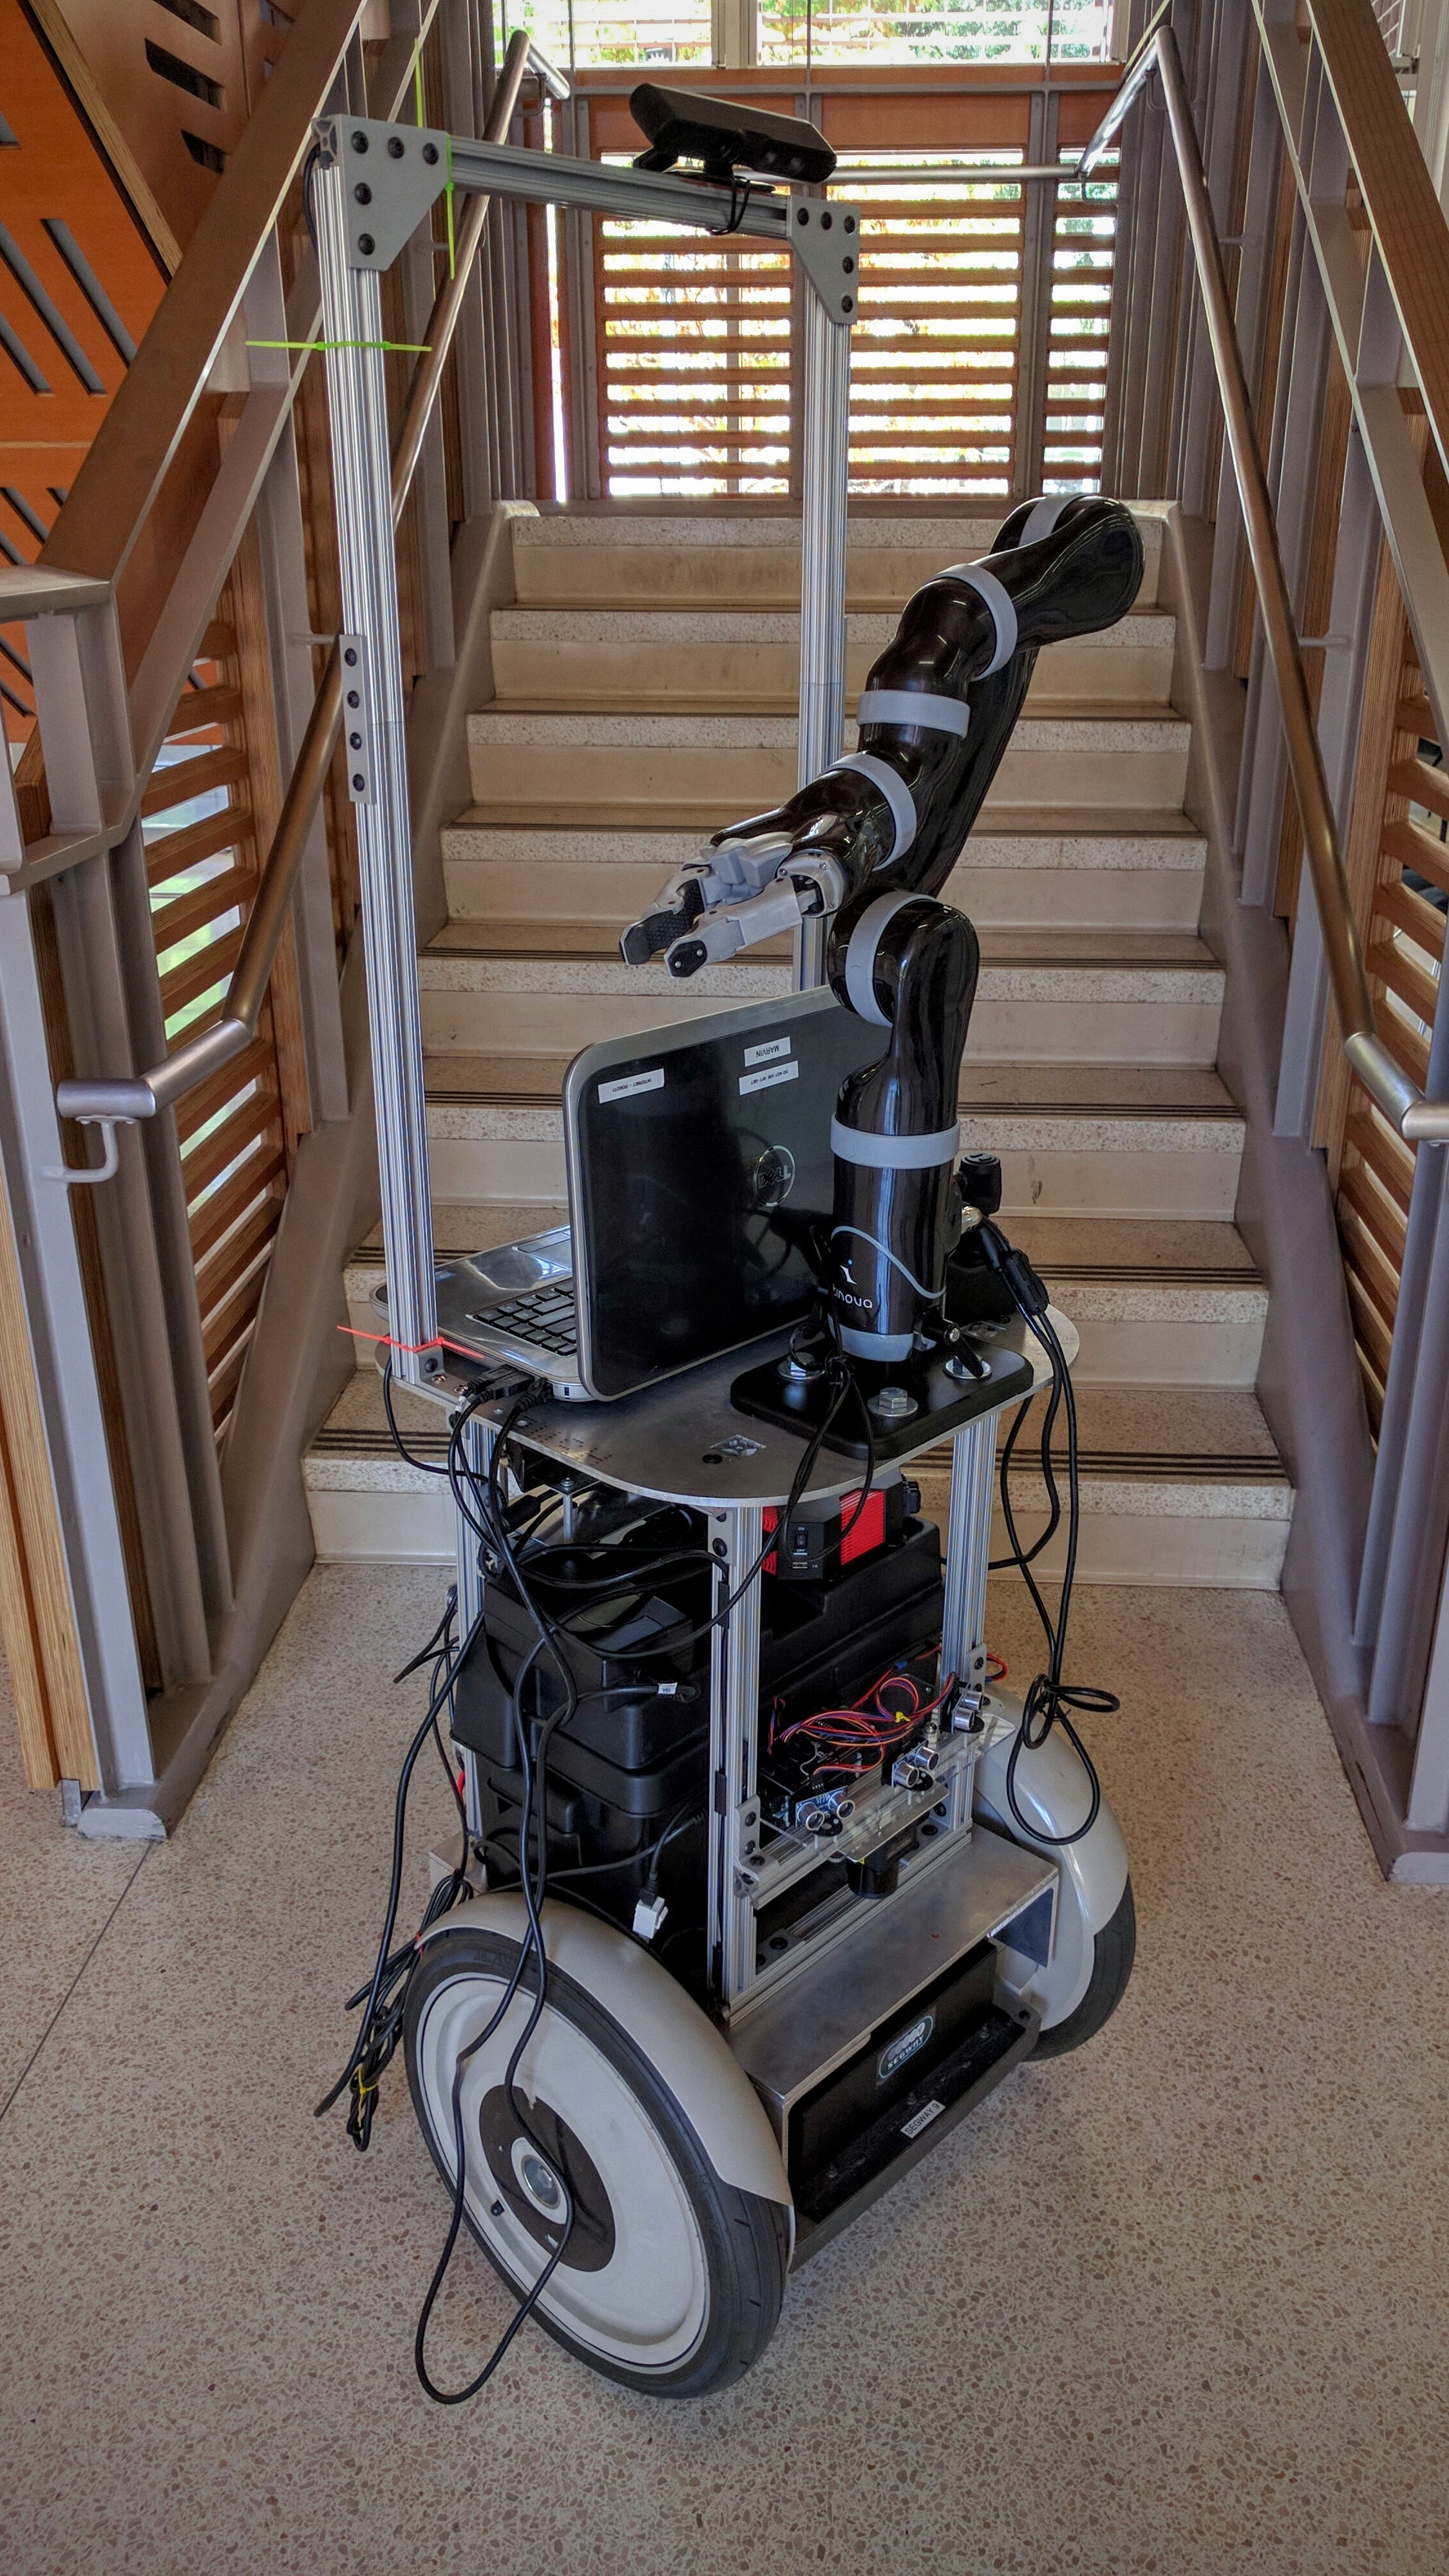
\includegraphics[width=\textwidth]{bwi_segbotarm}
    \caption{Segbot arm}
    \label{fig:segbotarm}
  \end{subfigure}
  \caption{The three active robot platforms in the BWI Lab}
  \label{fig:robots}
\end{figure}

\subsection{Hardware Platform}

All of our robots are powered by the Segway Robotics Mobility Platform (RMP).
Our latest generation robot uses the newer RMP 210 version, which comes with two
integrated lithium-ion batteries and can navigate at speeds up to 8
m/s and carry up to 45 kg of payload. The frame was designed in-house
and supports a large number of sensors. For navigation, localization, and
obstacle avoidance, we use a Velodyne VLP-16 Puck LIDAR. Point clouds (3D voxel
map) and video data are provided by an Xtion Pro, a device very similar to the
Microsoft Kinect. Our latest generation robots also have an additional Hokuyo
URG-04LX laser range finder to compensate for the LIDAR's blind spots. The
robot is equipped with a custom-built computer\footnote{3.9Ghz i7 processor,
16GB ddr3 RAM, Gigabyte GA-Q87TN motherboard, HDPLEX H1.S heatsink case, and a
Acer FT200 monitor} which runs Ubuntu 14.04. The computer is powered by the
RMPs battery, thus removing the need for an external car battery (which was
present in our Version 2 robots). The battery life on a running robot is
approximately 6 hours when actively using the base for navigation, and 10 when
stationary.

\subsection{Software Stack}

Our robots's software architecture is based on the Robot Operating System (ROS)
built by \citet{quigley2009}, which provides us with both the infrastructure to
run our robots as a distributed node system as well as the messaging framework
to connect all the different components together. ROS also provides us with
access to many community packages, such as device drivers, navigation
implementations, and planning systems.

Our robots use a hierarchical task-planning architecture for navigation
planning \citep{zhang2014}. A navigation request begins with the logical
planner, which uses Answer Set Programming (ASP) to describe the environment
\citep{lifschitz2008} -- such as which corridors connect with which hallways,
and which doors are open -- and then uses the ASP solver CLINGO to generate
possible plans \citep{gebser2014clingo}. It then moves to the logical navigator
which uses current and previous laser readings (in the form of occupancy maps)
and what it knows about the environment to create the navigation plan. Finally,
the local planner uses the immediate sensor readings to send commands to the
segway base and avoid any obstacles.

Almost all of the software that runs on our robots is open source. Furthermore,
all of the code that we write is also open source and available in the public
domain\footnote{\url{https://github.com/utexas-bwi}}. Our software is also
released as ROS packages back to the community and is available to install as
binaries.\footnote{\url{http://wiki.ros.org/bwi} and
\url{http://wiki.ros.org/segbot}}

\subsection{BWI Related Work}

The BWI lab has done extensive work on the planning and learning of action
cost. This enables our robots to plan high-level tasks such as navigating to
floors using hierarchical planning \citep{yang2014, khandelwal2014}. Using the
robot's point-cloud sensors \citet{gori2015robot} developed a system to perform
human activity recognition. \citet{khandelwal2015, khandelwal2014multi} have
also developed systems for multi-robot guidance that enable our robots to guide
humans to their desired locations. The segbot arm robot has also allowed the
lab to develop systems for grounded language learning by playing a game of I
Spy \citep{thomason2016} as well through human-robot dialog
\citep{thomason2015learning}. Similarly, the robot arm was used to perform
object exploration and ordering using haptic exploratory behaviors
\citep{sinapov2016}.

\section{The Web Client}\label{sec:client}

Virtour consists of two platforms: the user facing client, and associated
software that runs on the robots. The user client is accessible from a web
browser and is built using modern web frameworks to adhere to current web
development standards and simultaneously support as many platforms as possible.
We decided to use a web-based client because of the increasing prominence of
web browsers in people's lives. Furthermore, a web based approach means that
our end-users do not have to install any additional software to connect with or
use the robots, thus reducing the friction for using our system.

\subsection{Client Architecture}

The web client was developed using HTML5 and CSS3 to create the visual
interface and JavaScript to provide the functionality and connectivity. The
web client consists of multiple handlers and ROS clients which are used to
communicate with individual robot components such as the tour manager and
navigation managers. All ROS requests are routed through
roslibjs\footnote{\url{http://wiki.ros.org/roslibjs}} which serializes them and
uses a SOCKET connection to send them to the robot. The image and video
streaming are done without roslibjs for optimization reasons and are two
separate connections to the robot. In total, the web client communicates to the
robot using three different connections. The hierarchy of components and connections
can be seen in Figure \ref{fig:client}. 

\begin{figure}[t!]
  \centering
  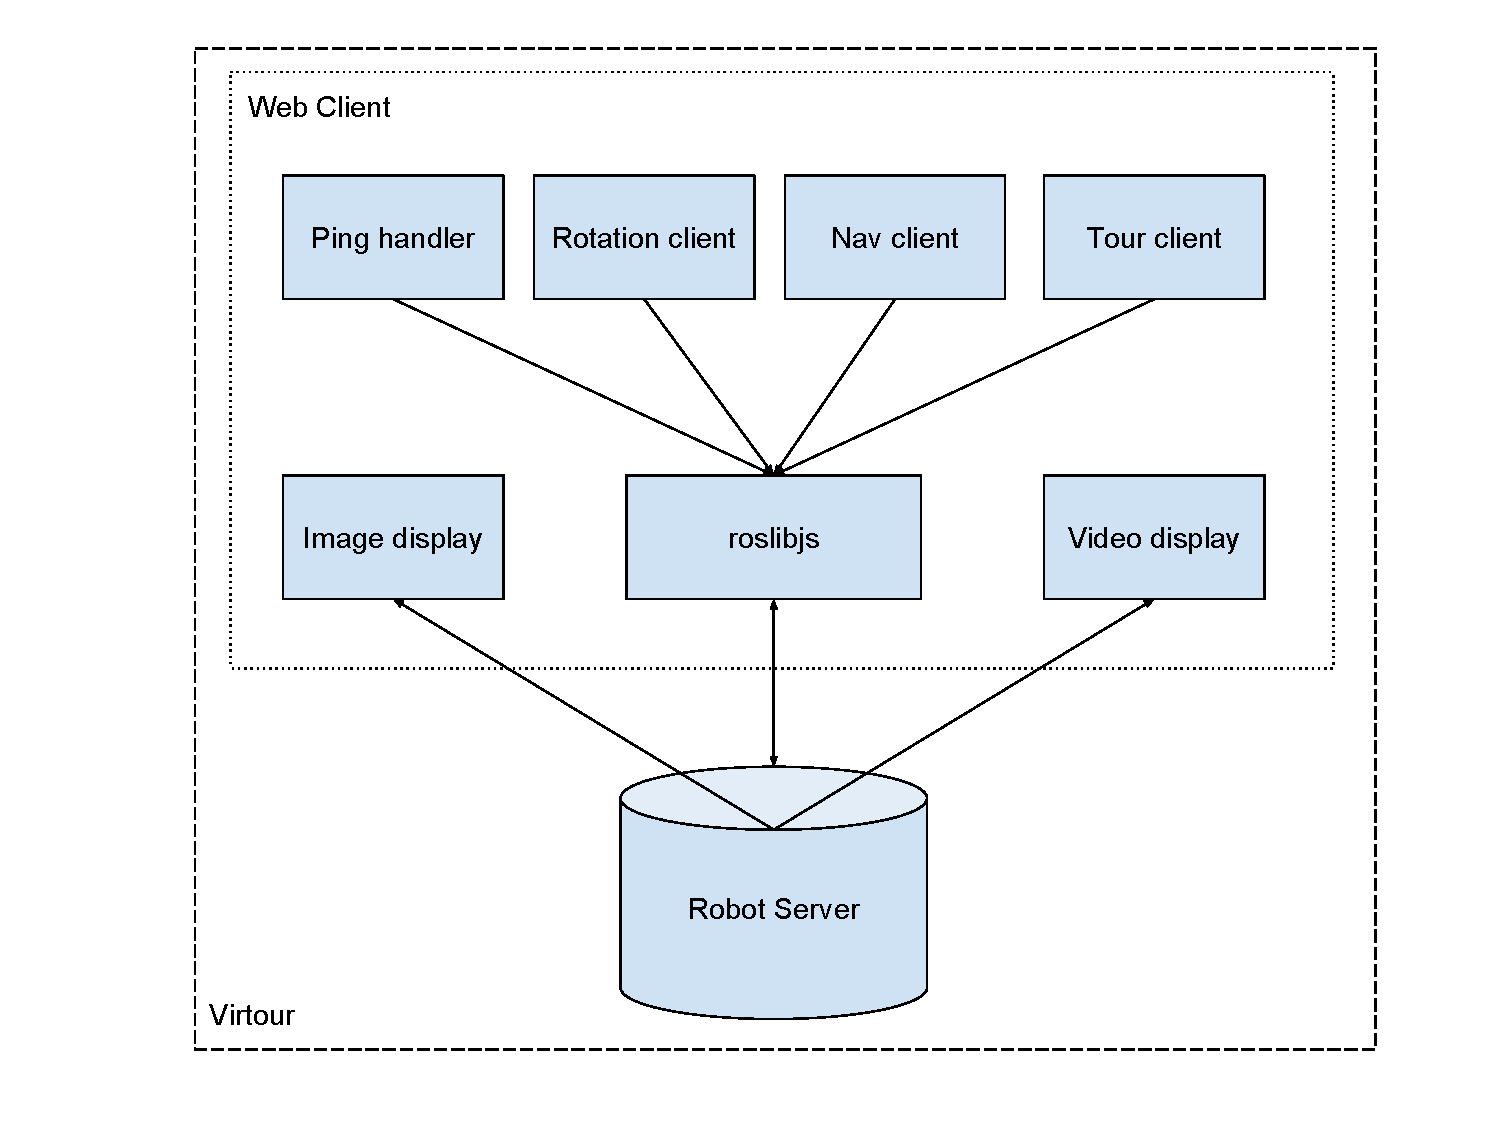
\includegraphics[width=0.95\textwidth]{virtour_client}
  \caption{Overview of the Virtour client structure and hierarchy of
  communication between the different components}
  \label{fig:client}
\end{figure}


\subsection{Modern Approach}

The web client is designed to be simple and functional while still being
aesthetically pleasing to end users. It uses a grid system powered by the
popular front-end library Bootstrap
2.0\footnote{\url{https://getbootstrap.com/}} to create a fully responsive web
layout. This allows us to support any web-powered platform (e.g., mobile
devices, tablets, and computers) by making the website scale and re-organize
based on the specifications of the device such as the screen resolution and
screen size. An example of responsive scaling can be seen in Figure
\ref{fig:homepage}.

When on the website, the user is greeted by a list of our currently active and
available robots (as seen in Figure \ref{fig:homepage}). Each robot is
represented by a name and associated picture. From here, a user can select a
robot to connect to by clicking on the robot's name or image. When the user
clicks on the robot, the web client will initiate a tour request to the
specified robot.  If the connection is successful the client will switch into a
tour session.

Tour sessions can be either led or spectated. When spectating, the user has no
control over the robot but can see the video stream, robot status, and the
location of the robot on the map in real time. When leading a tour the user can
actively instruct the robot to perform operations. Each tour can have at
most one leader, but no limit to the number of spectators. We built Virtour
this way to ensure there is a consistent leader experience (to avoid tour
contention by multiple users), and for security reasons, since we can control
whether a leader is allowed or not. If the tour has no existing leader and
tours are allowed then a visiting user can choose to become tour leader by
pressing the ``Become Leader'' button. Upon success, it will present the user
with the leader user interface (UI).

\begin{figure}[!tbp]
  \begin{subfigure}[b]{0.63\textwidth}
    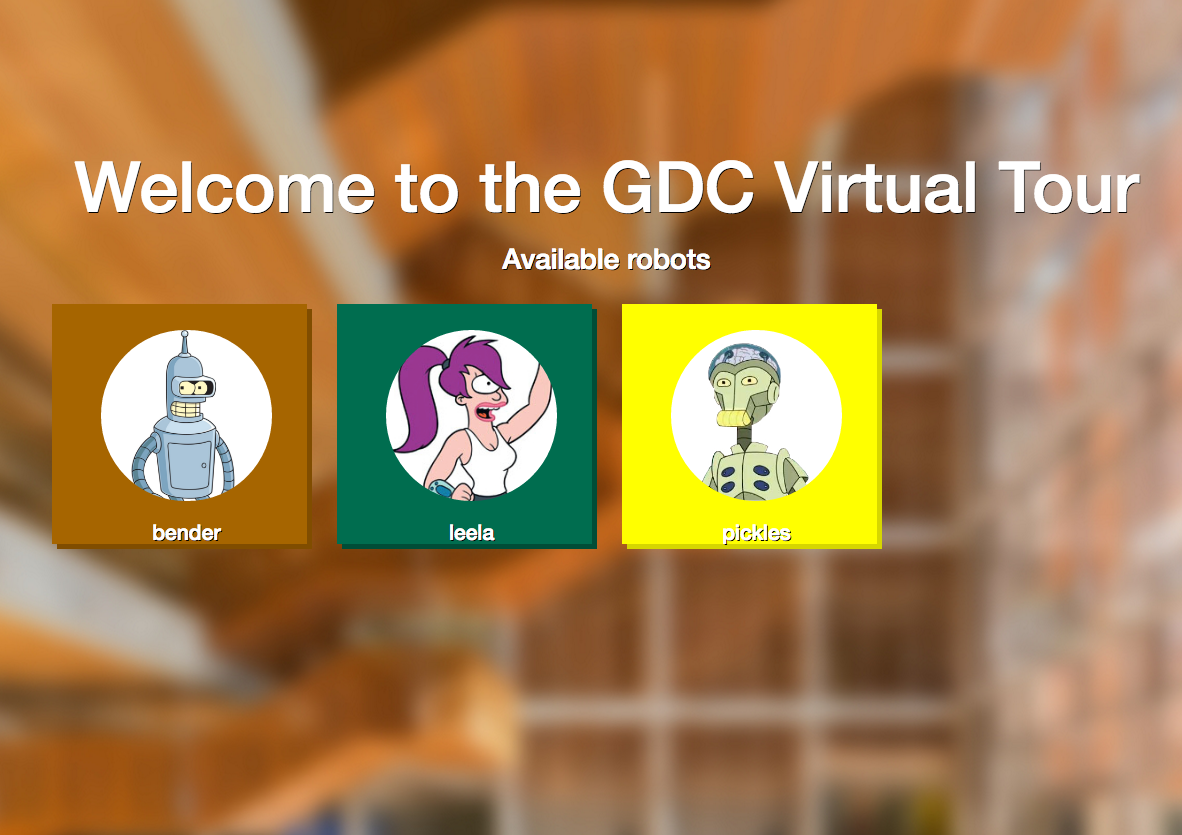
\includegraphics[width=\textwidth]{tour_homepage}
    \caption{Desktop view}
  \end{subfigure}
  \hfill
  \begin{subfigure}[b]{0.25\textwidth}
    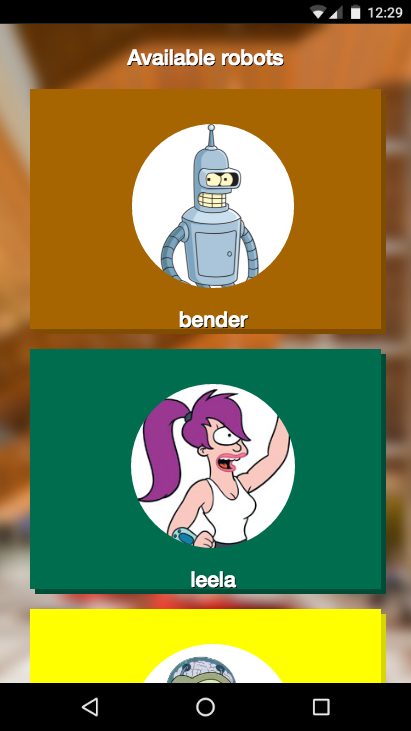
\includegraphics[width=\textwidth]{mobile_homepage}
    \caption{Mobile view}
  \end{subfigure}
  \caption{Landing page whenever someone visits the website, from here users
  can select which robot to connect to}
  \label{fig:homepage}
\end{figure}

\subsection{Leader User Interface}

\begin{figure}
  \centering
  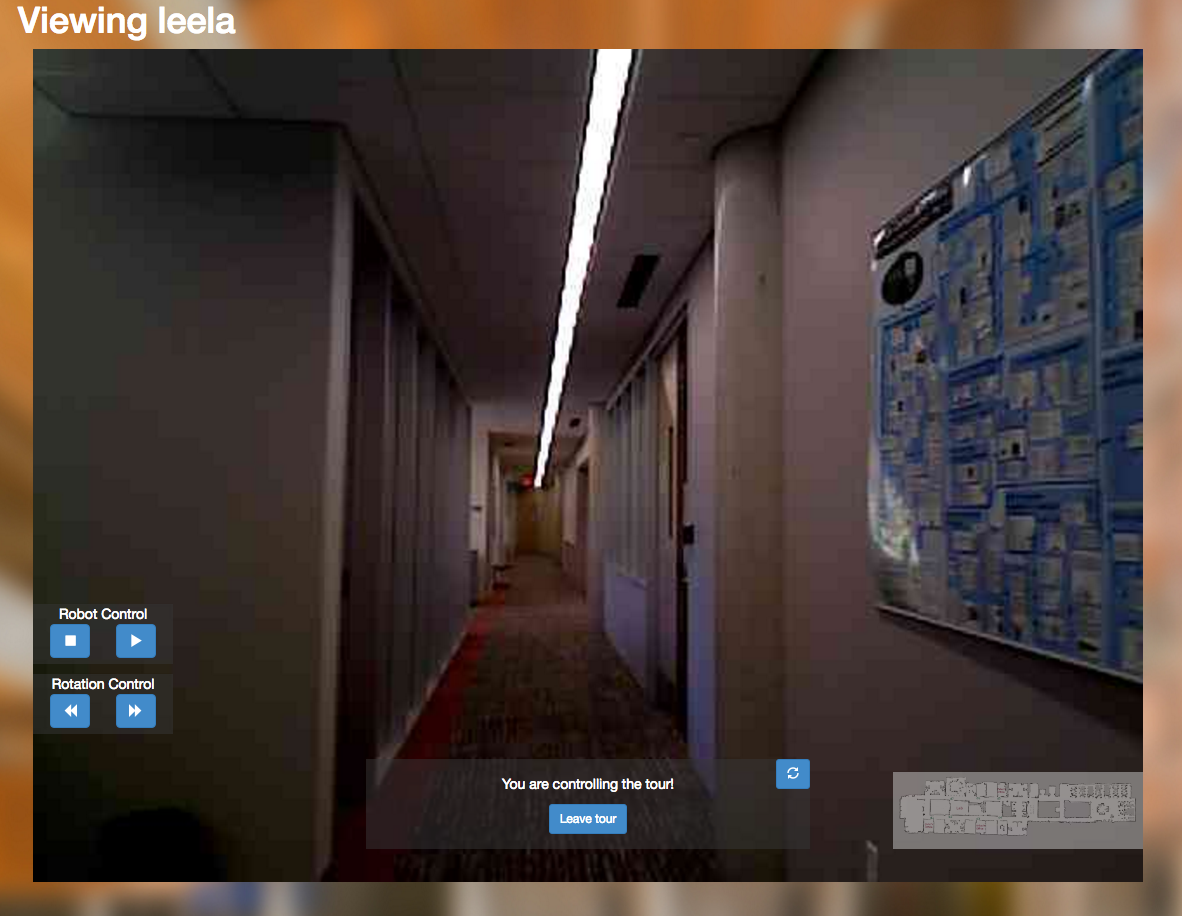
\includegraphics[width=0.95\textwidth]{leader_ui}
  \caption{The controls available to the leader whenever they are leading a
  tour}
  \label{fig:leader_controls}
\end{figure}

The leader UI adds a number of components to that allow the user to control the
operations of the robot. The list of available remote-control capabilities is
as follows:

\begin{itemize}
  \item Rotate the robot
  \item Navigate to a room 
  \item Navigate to a door 
  \item Speak a message (using text-to-speech)
  \item Deliver a spoken message (using text-to-speech) to a location
  \item Pause and resume a scavenger hunt task
  \item Move the robot's pan/tilt camera unit
\end{itemize}

\begin{figure}
  \centering
  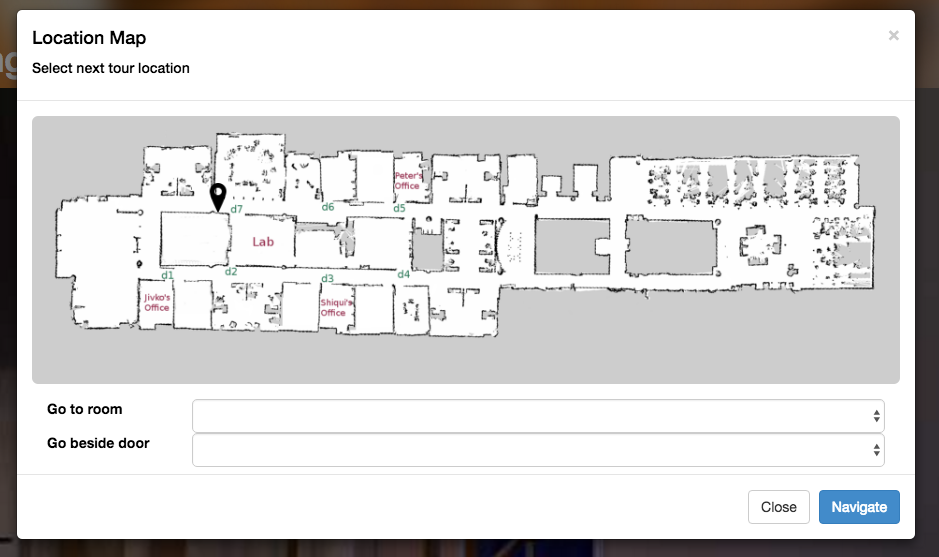
\includegraphics[width=0.95\textwidth]{nav_ui}
  \caption{Navigation interface for leaders which is displayed whenever the
  mini map is pressed, from here they can select a room or door to navigate to}
  \label{fig:nav_interface}
\end{figure}

The user can interact with the interface to request any of the tasks. For
example, whenever the user is the leader, a pair of directional arrow buttons
is shown which will immediately rotate the robot when pressed. Navigation
commands are accessed within the navigation pane which can be accessed by
clicking on the mini map.

Whenever a user first connects to a robot, the web client will query the robot
for the capabilities that it has (e.g., which generation robot, which cameras it
has access to, if the camera has servos, etc) and then adapt the user
interface accordingly to support whichever robot the user is connected to.

To maintain leader consistency, the leader UI will ping the server at
a known interval to ensure the leader is still connected. This allows the
server to become aware of a dropped connection. Thus, if the user closes the window
or the ping fails, the leader will relinquish the leader status so other users
can control the robot.


\subsection{Guest User Interface}

\begin{figure}
  \centering
  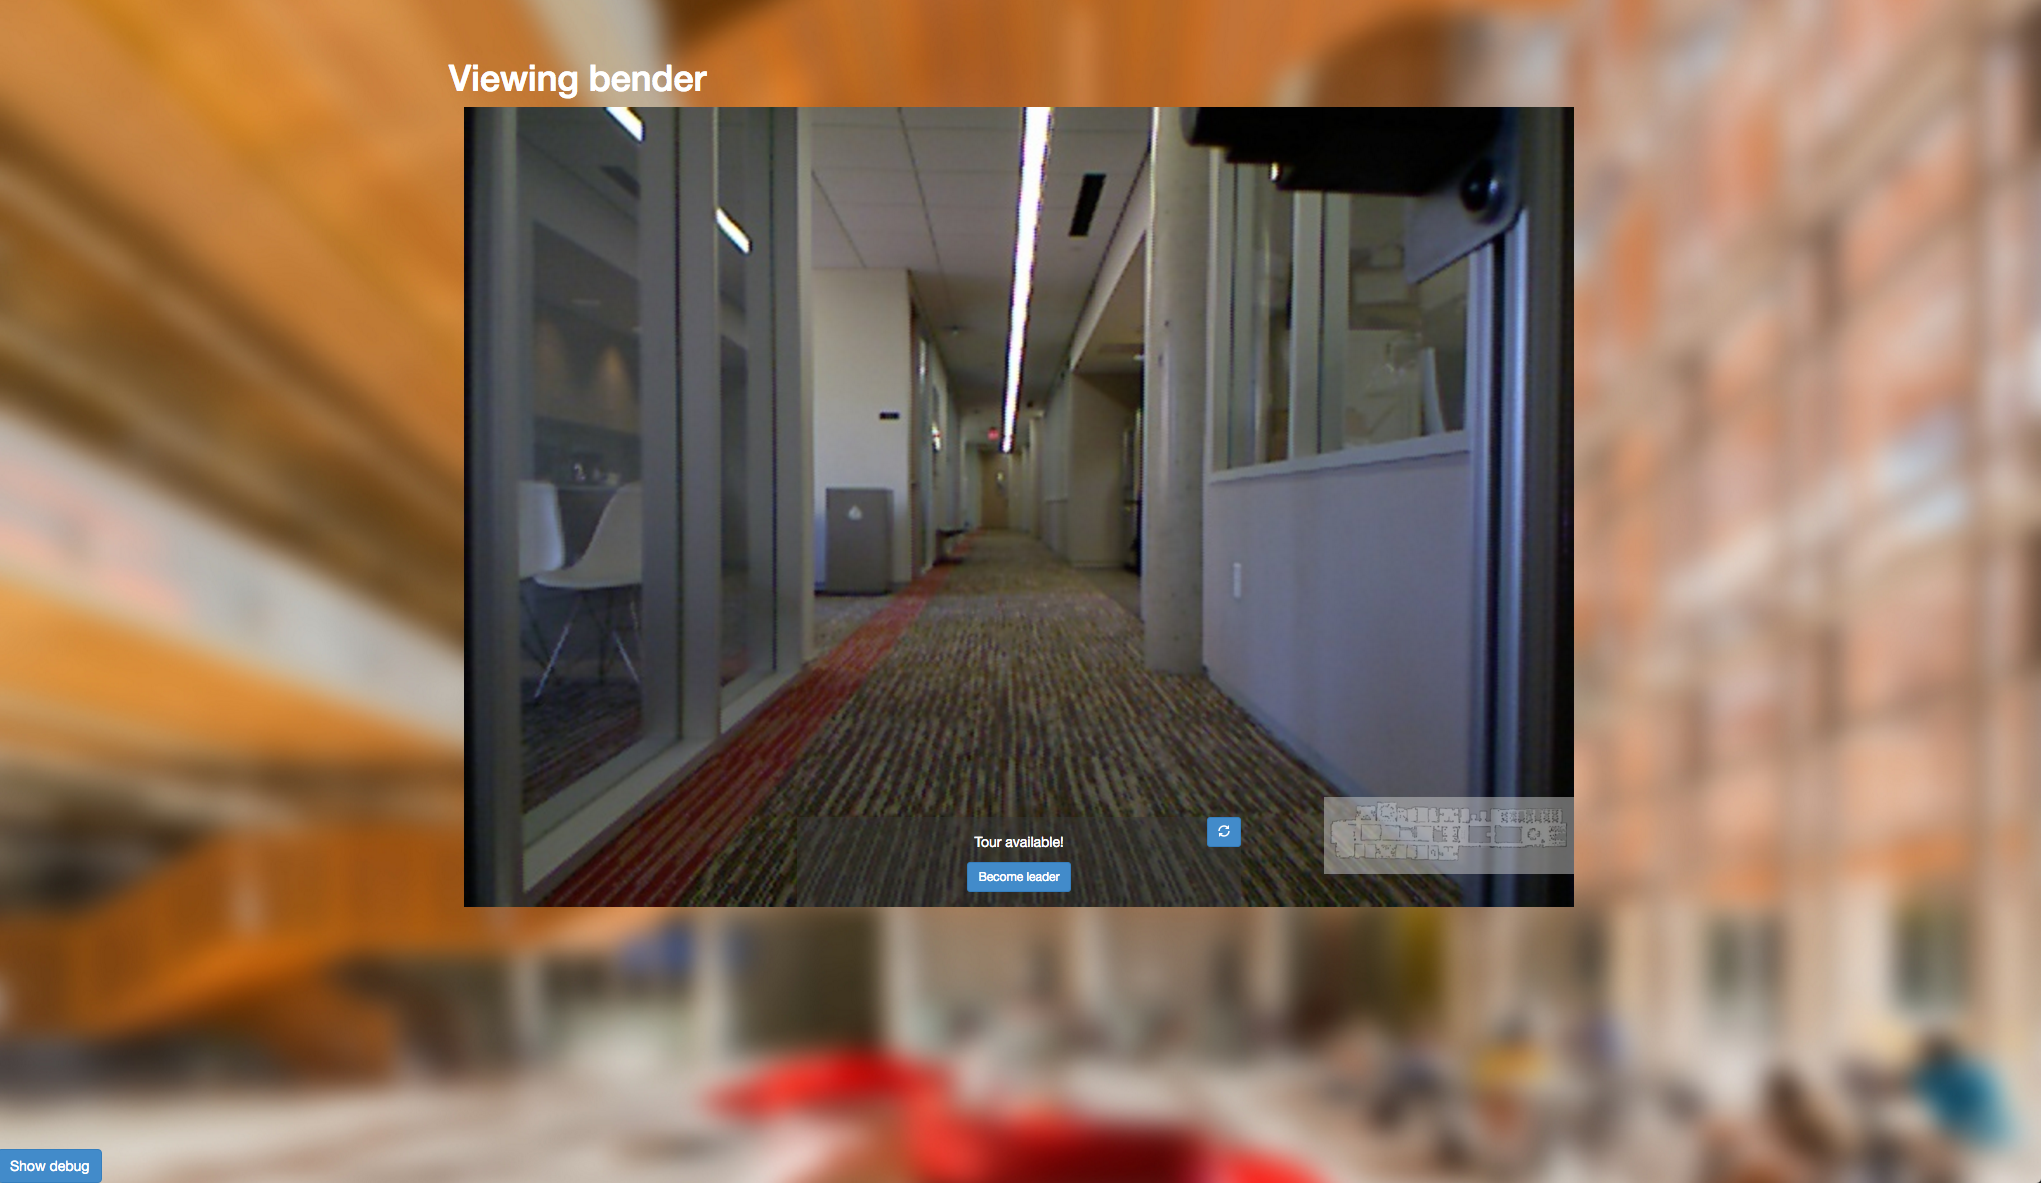
\includegraphics[width=0.95\textwidth]{guestUI}
  \caption{What a user might see whenever they connected to a robot but are not
  the tour leader}
  \label{fig:guest_mode}
\end{figure}

The guest UI is the default interface presented to the user whenever he or she
connects to a robot. The predominant view is the live stream from the robot's
camera, which is shown in the center. The robot's camera is placed
strategically so as to provide the user with the robot's point of view. This
makes the user experience more realistic and makes the tour more engaging.

The interface also displays a mini map of the floor the robot is
on, with a marker to indicate the robot's current position.  If the
robot navigates to another floor (via the elevator), Virtour will recognize the
floor change and show the most up-to-date map of the current floor.

Finally, the guest UI has a status box which displays whether or not a tour is
ongoing, allowed, or disabled. From here the user can request to become tour
leader (if available), or wait for a tour to be available. All our robots have
the guest UI enabled at all times, so that users can remotely connect to the
robots and experience what they are doing. For privacy reasons, the robot will
have turn on indicator lights (using the mounted individually-addressable LED
strips) whenever there is someone streaming video (at the moment only supported
in our latest generation robot).


\section{The Server}\label{sec:server}

\begin{figure}
  \centering
  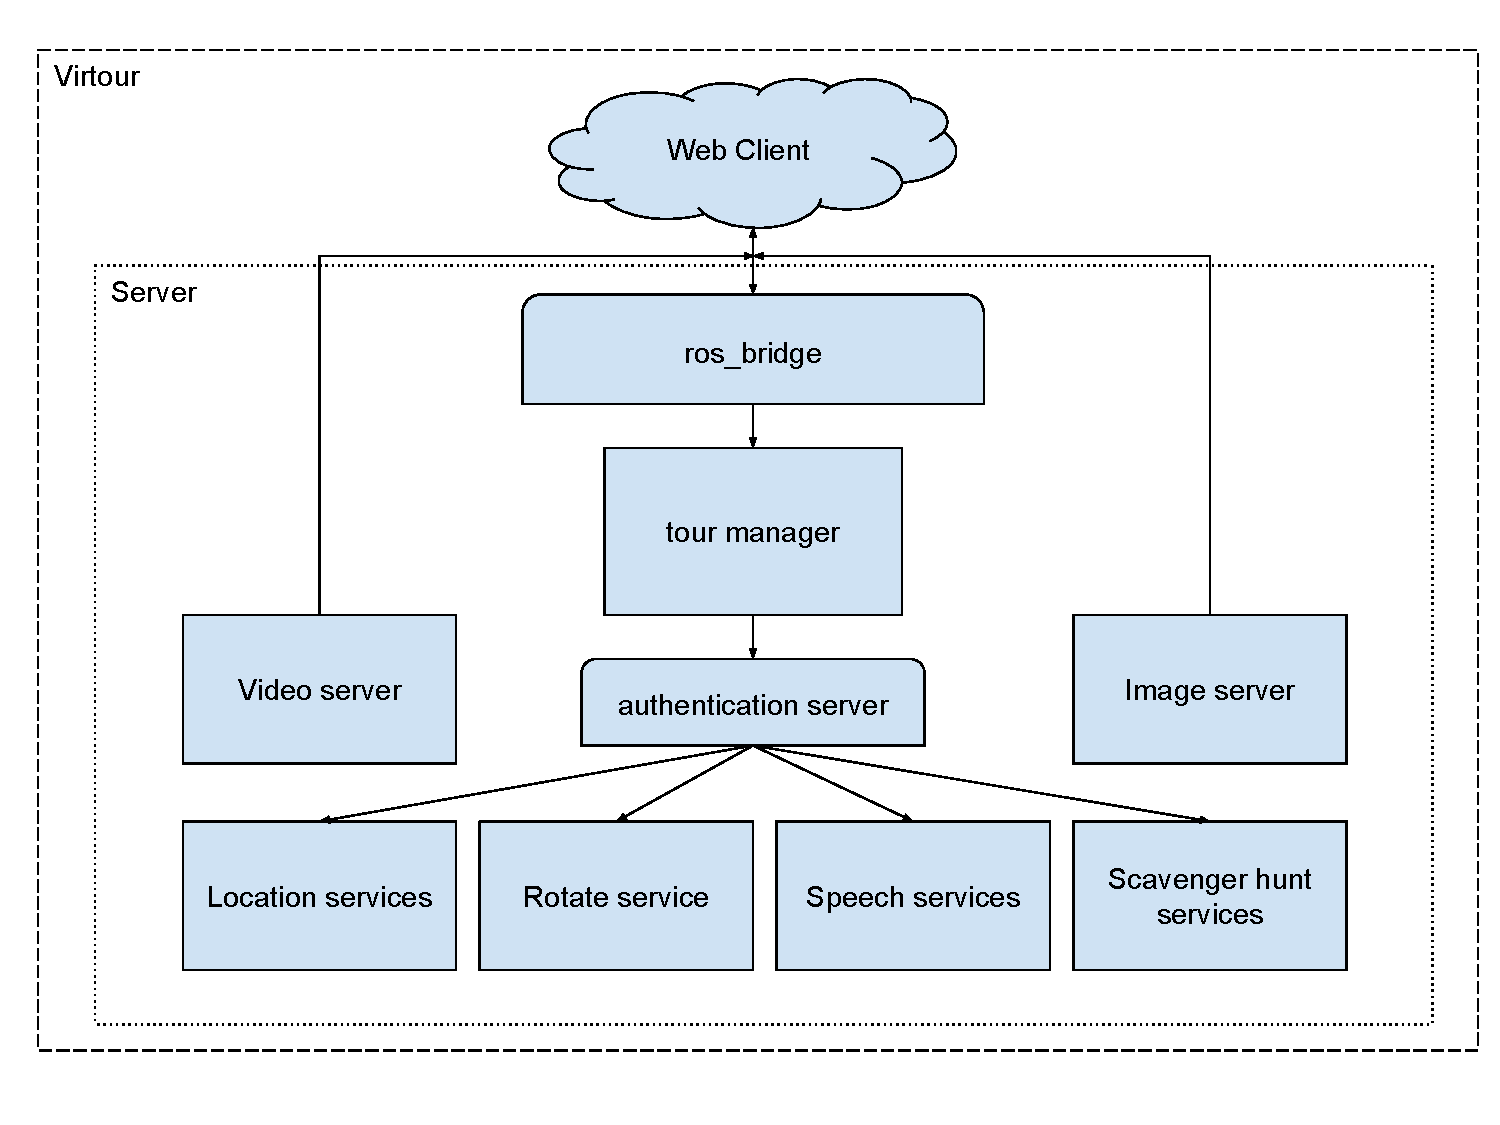
\includegraphics[width=0.95\textwidth]{virtour_server}
  \caption{Overview of the Virtour server structure and hierarchy of
  communication within the server nodes and the web client}
  \label{fig:server}
\end{figure}

The server consists of a number of components which run on the physical robot
to enable the web client to perform the required operations. Most communications
from the web client go through the ROS bridge node, which is responsible
for translating the serialized socket commands to normal ROS commands. This is
the case for all action requests and commands. From there, requests are
sent to the tour manager, which will authenticate the requests (to ensure they
are validly formed and come from an accepted source) and then delegate them to
their respective service providers. The robots also have two other open
connections for streaming images and video to web clients. The hierarchy of
communications can be seen in Figure \ref{fig:server}.

\subsection{Tour Manager}

The tour manager serves the role of maintaining tour integrity and managing
active connections with all the clients that are connected to the robot. It
maintains of an internal state machine to keep track of whether tours are
enabled and, if so, whether one is active. It will also maintain connection
with the tour leader through pings to ensure the leader remains alive. If the
leader disconnects (by closing the page) or is disconnected (missing a ping),
the tour manager will demote them and make tour leadership available again. The
tour manager is also responsible for granting tour leader status to clients
that properly request it whenever tours are enabled.

\subsubsection{Robot Control}

The server-side code powering the remote robot control consists of various
service providers which use the tour manager to authenticate requests, and then
translate them to the appropriate robot commands. For example, the rotate
control will take the rotate command (if properly authenticated) and then
translate it to raw segway base navigation commands. Message delivery and
speaking requests will be routed to their appropriate service providers.
Similarly all door or room navigation requests will go to the logical planner
in the form of ASP goals. For example, a request to navigate to a specific
office will be turned into an ASP goal such that it is impossible for the robot
to not be in that location. The navigation and planning stack then take over
and will perform the planning and navigation required to accomplish the goal.

\subsection{IP management}

In order to manage the IP addresses of all the robots, we created
smallDNS\footnote{Source code is available at
\url{https://github.com/pato/smallDNS}} (small multi-agent locally listable
DNS). SmallDNS keeps track of the IP addresses of each of the robots (which are
dynamically assigned and thus change from time to time). Furthermore, it also
keeps track of which robots are available and running via series of pings. This
means that the end user does not need to worry about the changing IPs of the
robots or which ones are alive. So when the user visits the home page (Figure
3), they will see the list of currently active robots and will be able to
connect to each without having to know the IP address.

SmallDNS consists of a simple DNS server running on our master server, which is
accessible from all our robots. The server was written in Python and can
handle HTTP requests. It can respond to update requests whenever a robot has
a new IP address, as well as conventional GET requests to display the list of
robots over text or JSON\footnote{JavaScript Object Notation - a human-readable
data-interchange format}. It stores everything in-memory for performance
reasons, but will write it to disk periodically so that we do not lose
information in case the server is stopped.

Each of the robots has a bash script which checks the robot's IP address against the
last update IP address to see if there is a change. If the IP has changed, the robot
will perform an update request on the server to inform it of the new address. This
script is configured using a cronjob which runs every three minutes.

\section{Security and Safety}\label{sec:security}

Security was a top concern in designing Virtour since the system allows
external parties to remotely operate our robots. Our two main security
objectives were to prevent unapproved or harmful interactions with the robots
and to prevent unauthorized access to Virtour. Furthermore, since the robots
are physically navigating potentially crowded spaces, we wanted to make sure
that safety was a top priority.

\subsection{Client Side}

The client works to prevent unapproved interactions by only presenting the user
with ability to interact with the robot in the approved behaviors. On the
JavaScript client-side, we also only create service and action clients (the
communication methods that are used to request actions on the robot) that
perform specific tasks, rather than general-purpose clients. This reduces the
likelihood of an end-user issuing unapproved commands. To identify users, each
client is assigned a universally unique identifier (UUID) which is used to
authenticate all communication with the robot.

\subsection{Server Side}

For security reasons, we only allow outside parties to become leaders (and thus
have control of the robot's operations) if we explicitly enable virtual tours
on the robot. Unlike the guest UI which is enabled any time the robot running,
the server implementation of leader control is disabled by default to prevent
unexpected access. Furthermore, all operations which affect the state of the
robot (ie: rotating and navigating) require proper authentication. The server
keeps track of the UUID of the currently active leader, and will only grant
that specific client the ability to control the robot. This prevents
unauthorized users from executing actions on the robot. To prevent denial of
service by any one leader (by not relinquishing their leadership or dropping
the connection), the server uses the ping system to ensure that the leader is
alive and connected. Furthermore, there is a 15 minute time limit per leader,
to avoid a single leader taking perpetual control of the system. Finally, we
always have the option to disable tours (via the tour manager) which will
immediately evict any active leaders and revoke all remote control of the
robot.

Safety for users and the robot is ensured through the use of shared autonomy.
Whenever users request navigation to locations via the client UI, the robot
will perform the navigation using the full navigation stack which includes the
global planner and local obstacle avoidance. Furthermore, the server
has a whitelist of pre-approved locations the users can request on the
client which it uses to verify all navigation requests, to prevent navigation
to incorrect or invalid locations. Finally, because of the way rotation is
implemented, the robot stays entirely within its footprint when it rotates.
When combined with the safety of our navigation stack, this means that in-place
rotation is always safe.


\section{Scavenger Hunt Integration}\label{sec:scav}

\begin{figure}
  \centering
  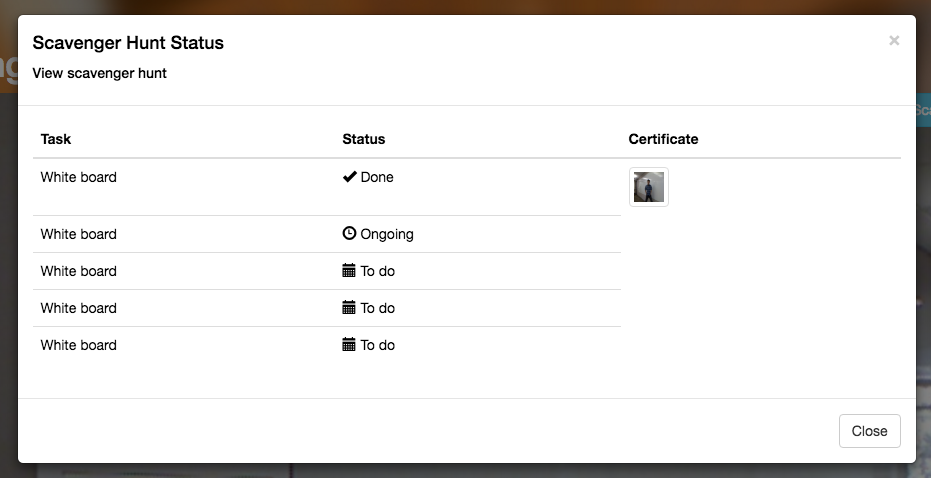
\includegraphics[width=0.95\textwidth]{scav_certs}
  \caption{The scavenger hunt task list displays all the active tasks along
  with their status, and if complete will allow the user to view the
  certificate}
  \label{fig:scav}
\end{figure}

In addition to the remote control capabilities available through our website,
Virtour was also fully integrated with the Robot Scavenger Hunt
by \citet{zhang2016}.  The Robot Scavenger Hunt is a framework of tasks that AI
capable robots can complete autonomously. These are used to
evaluate and compare the performance of autonomous robots that reside in larger
spaces and operate autonomously for long durations of times. We supported all
four tasks in the task library, which require the robot to find a human wearing
a specific colored shirt, to follow a human for more than 10 meters, to deliver
a given object, and to find a specific object. All four of these task
variations require a certificate of work which are images of the task being
accomplished (e.g., a picture of a human wearing a blue shirt). Whenever a
robot participates in the scavenger hunt, it is assigned a random set of daily
tasks that it must then work to finish that day.

Whenever a user uses Virtour to connect with a robot running the scavenger
hunt, Virtour will detect the scavenger hunt and allow the users to interact
with the scavenger hunt. For example, the user can see the list of the
currently running tasks by clicking on the scavenger hunt button. The
server-side portion of Virtour comes integrated with an HTTP image web server
which is used to provide the user interface with images of the complete tasks, 
so if available, Virtour will display the certificates on the website as
thumbnails on the scavenger hunt task list (illustrated in Figure
\ref{fig:scav}) but they can expanded to see the full-size image by clicking on
them. Finally, if the user is the leader, they can also control the operation
of the scavenger hunt by stopping and resuming the current task. This allows a
user to stop the current scavenger hunt task, then navigate the robot elsewhere
or perform any other supported operation, and resume the scavenger hunt later.

\section{Conclusions and Future Work}\label{sec:conclusion}

In this paper, we introduced a novel telepresence system which gives users
shared autonomy over the control of our robots. This system allows users to use
their common internet-powered devices to access the Virtour website. The
Virtour website allows users to securely join an existing tour as spectators,
or, if available, to optionally lead a tour. This would give them the ability
to make the robot navigate to desired locations and doors, as well as deliver
messages, or perform scavenger hunt tasks. Users can experience the tour
through the on-board camera which is streamed dynamically to the website as
well as to track the robot's movement using the real-time map.

Further work could extend the navigation system to allow the users
point-and-click navigation to arbitrary points, while still maintaining shared
autonomy. There is also work in adding more ways for remote users to interact
with the robot's environment, such as using actuators or interacting via a
mounted arm on the robot. There are multiple other ways of improving the client
user interface such as adding the display of other information such as distance
traveled or battery level information.

Finally, although our focus has been on remotely operated building tours,
Virtour has laid the groundwork for a more complete telepresence robot system
which could target other commercial uses such as hospitals (for family visits,
or nurse checkups), as well other research-oriented projects such as HRI
studies or robot monitoring systems. Most of our work is directly applicable
and can be tailored to many different uses, since the communication,
authentication, and interaction protocols that Virtour uses can be used
independently.

\section{Acknowledgments}\label{sec:acks}

Virtour could not have been accomplished without the guidance and support of my
original research advisor Matteo Leonetti, and my current research advisors
Jivko Sinapov and Peter Stone. Shiqi Zhang for helping with the scavenger hunt
integration. Maxwell Svetlik for insightful comments and support throughout the
project, Walter Sagehorn for helping develop smallDNS and to Benjamin Singer
for developing the message delivery tasks.

%\nocite{*}
\bibliographystyle{apacite}
\bibliography{citations}
    
\end{document}
